\documentclass{article}
\usepackage{amsmath}
\usepackage{amsfonts}
\usepackage{amssymb}
\usepackage{hyperref}
\usepackage{graphicx}
\usepackage{float}
\usepackage[margin=1in]{geometry}

\title{Parametric \& Nonparametric Statistics Project}
\author{Aleksandr Jan Smoliakov}
\date{2024--12--12}

\begin{document}

\maketitle

\section{Introduction}



\section{Preliminaries}

In the project below, we will use the following parameters:
\begin{itemize}
    \item $\mathcal{N} = 9$ (first name: `Aleksandr', 9 letters)
    \item $\mathcal{S} = 9$ (last name: `Smoliakov', 9 letters)
    \item $\mathcal{I}_1 = 5$ (last digit of study book number)
    \item $\mathcal{I}_2 = 8$ (second last digit of study book number)
\end{itemize}

Let \(G_1, \ldots, G_m\) be given distribution functions and \(p_1, \ldots, p_m\) be probabilities that sum to 1. The distribution function \(G\) defined by

\[
G(u) := p_1 G_1(u) + \cdots + p_m G_m(u) = \sum_{k=1}^m p_k G_k(u), \quad u \in \mathbb{R}
\]
is called a mixture of distribution functions \(G_1, \ldots, G_m\) with probabilities (or weights) \(p_1, \ldots, p_m\).

\(G\) is the distribution function of the random variable \(Z\) generated in the following way:

\begin{enumerate}
    \item Choose \(k \in \{1, \ldots, m\}\) at random with probabilities (or weights) \(p_1, \ldots, p_m\). The chosen number is denoted by \(k^*\).
    \item Generate a random variable \(Z^*_{k^*}\) according to the distribution function \(G_{k^*}\) and assign \(Z \leftarrow Z^*_{k^*}\).
\end{enumerate}

In this task, we will have \(m = 2\), so the algorithm for generating \(Z\) is as follows:

\[
Z \leftarrow Z^*_{1+k^*} \quad k^* \sim \text{Binomial}(1, p_2), \quad Z^*_{k} \sim G_k \ (k = 1, 2).
\]

Let
\[
\mathcal{G}(\Theta) = \{G(\cdot|\boldsymbol{\theta}), \boldsymbol{\theta} \in \Theta\}
\]

be a given parametric family of absolutely continuous parametric functions \(G(\cdot|\boldsymbol{\theta})\) with the respective distribution densities \(g(\cdot|\boldsymbol{\theta})\) dependent on the unknown parameter \(\boldsymbol{\theta} \in \Theta\). It is assumed that \(\boldsymbol{\theta}\) is two-dimensional, i.e., \(\boldsymbol{\theta} = (\theta_1, \theta_2) \in \mathbb{R}^2\).

\subsection{Parametric Family Selection}

Using the assigned formula \( \ell := \left\lfloor \frac{\mathcal{I}_2 + 2.5}{2} \right\rfloor \), we find \( \ell = 5 \). Thus, we will use the parametric family \(\mathcal{G}_5(\Theta)\) in this task.

$\mathcal{G}_5(\Theta)$ contains distribution functions of random variables uniformly distributed on $[\theta_1, \theta_2]$, where $\theta_1 < \theta_2$.

It can be expressed as:
\[
G(u|\boldsymbol\theta) = \begin{cases}
0 & u < \theta_1 \\
\frac{u - \theta_1}{\theta_2 - \theta_1} & \theta_1 \le u \le \theta_2 \\
1 & u > \theta_2
\end{cases}
\]
with \(\boldsymbol\theta = (\theta_1, \theta_2) \in \mathbb{R}^2\) and \(\theta_1 < \theta_2\).

\section{Task 1: Testing Goodness-of-Fit}

\subsection{Basic Distribution Function}

The problem gives a specific basic parameter:
\[
\boldsymbol\theta_0 = (-\mathcal{N}, \mathcal{S} + 4) = (-9, 13).
\]

Thus, the basic distribution function is:
\[
G_0(u) = \mathcal{G}_5(u|\boldsymbol\theta_0) = U(-9, 13).
\]

For a uniform distribution \(U(a,b)\):

\begin{itemize}
    \item Mean: \(\mu = \frac{a+b}{2}\)
    \item Variance: \(v^2 = \frac{(b-a)^2}{12}\)
\end{itemize}

For \(G_0 = U(-9, 13)\):

\[
\mu_0 = \frac{-9 + 13}{2} = \frac{4}{2} = 2
\]

\[
v_0^2 = \frac{22^2}{12} = \frac{484}{12} = \frac{121}{3} \approx 40.3333
\]

\subsection{Finding Mixture Distributions}

We are given the following equations for the mixture distributions \(G_1\) and \(G_2\):

\[
\mu_0 = \mu(\boldsymbol\theta_1), \quad \mathcal{N} v_0^2 = v^2(\boldsymbol\theta_1).
\]

\[
\mu_0 + 2v_0 = \mu(\boldsymbol\theta_2), \quad v_0^2 = \mathcal{S} v^2(\boldsymbol\theta_2).
\]

\subsubsection{Determining \(G_1\)}

First we determine \(G_1\). We have:

\[
\mu_0 = \mu(\theta_1), \quad \mathcal{N} v_0^2 = v^2(\theta_1).
\]

It is given that $\mu(\theta_1) = \mu_0 = 2$.

Plugging in \(\mathcal{N} = 9\) and \(v_0^2 = \frac{121}{3} \), we get:
\[
v^2(\boldsymbol\theta_1) = \mathcal{N} v_0^2 = 9 \times \frac{121}{3} = 363.
\]

Let \(G_1(u) = U(a_1, b_1)\). For a uniform distribution:
\[
\mu(\boldsymbol\theta_1) = \frac{a_1 + b_1}{2}, \quad v^2(\boldsymbol\theta_1) = \frac{(b_1 - a_1)^2}{12}.
\]

Since \(\mu(\boldsymbol\theta_1) = 2\):
\[
\frac{a_1 + b_1}{2} = 2 \implies a_1 + b_1 = 4.
\]

Since \(v^2(\boldsymbol\theta_1) = 363\):
\[
\frac{(b_1 - a_1)^2}{12} = 363 \implies b_1 - a_1 = \sqrt{(b_1 - a_1)^2} = \sqrt{4356} = 66.
\]

Solving the system:
\[
a_1 + b_1 = 4, \quad b_1 - a_1 = 66.
\]

Adding the two equations:
\[
2b_1 = 70 \implies b_1 = 35.
\]
\[
a_1 = 4 - 35 = -31.
\]

Thus:
\[
\boldsymbol\theta_1 = (-31, 35) \implies G_1(u) = U(-31, 35).
\]

\subsubsection{Determining \(G_2\)}

Repeating the process for \(G_2\). We have:

\[
\mu_0 + 2v_0 = \mu(\boldsymbol\theta_2), \quad v_0^2 = \mathcal{S} v^2(\boldsymbol\theta_2).
\]

Given \(\mu_0 = 2\) and \(v_0^2 = 40.3333\), we have:

\[
\mu(\boldsymbol\theta_2) = \mu_0 + 2v_0 = 2 + 2 \times \sqrt{40.3333} = 2 + 2 \times 6.3509 = 2 + 12.7018 = 14.7018.
\]

Also:
\[
v_0^2 = \mathcal{S} v^2(\boldsymbol\theta_2) \implies 40.3333 = 9 v^2(\boldsymbol\theta_2) \implies v^2(\boldsymbol\theta_2) = \frac{40.3333}{9} \approx 4.4815.
\]

For \(G_2(u) = U(a_2, b_2)\):
\[
\frac{a_2 + b_2}{2} = 14.7018 \implies a_2 + b_2 = 29.4036.
\]
\[
\frac{(b_2 - a_2)^2}{12} = 4.4815 \implies (b_2 - a_2)^2 = 4.4815 \times 12 = 53.7777.
\]
\[
b_2 - a_2 = \sqrt{53.7777} \approx 7.3333.
\]

Solving the system:
\[
a_2 + b_2 = 29.4036, \quad b_2 - a_2 = 7.3333.
\]

Adding the two equations:
\[
2b_2 = 36.7369 \implies b_2 = 18.3685.
\]
\[
a_2 = 29.4036 - 18.3685 = 11.0351.
\]

Thus:
\[
\boldsymbol\theta_2 = (-11.0351, 18.3685) \implies G_2(u) = U(11.0351, 18.3685).
\]

\subsection{Computing \( p_1 \) and \( p_2 \)}

Given:
\[
\tau = \frac{1}{1+I_1}, \quad I_1 = 5 \implies \tau = \frac{1}{6}.
\]
\[
\alpha_1 = 0.1, \quad \alpha_2 = 0.01.
\]

\[
p_1 = (\alpha_1)^{1-\tau} (\alpha_2)^\tau = (0.1)^{5/6} (0.01)^{1/6} \approx 0.06813.
\]

Then:
\[
p_2 = \frac{5 p_1}{\sqrt{S}} = \frac{5 \times 0.06813}{\sqrt{9}} = \frac{0.3406}{3} \approx 0.1135.
\]

\subsection{Determining Mixture Distributions}

We consider testing:
\[
H_0: F_Y = G_0 \textbf{ versus } H': F_Y \neq G_0
\]

We will compare the empirical distribution of samples generated from:

\begin{enumerate}
    \item \(F_Y = (1-p_1)G_0 + p_1 G_1\), i.e. a mixture of \(G_0\) and \(G_1\).
    \item \(F_Y = (1-p_2)G_0 + p_2 G_2\), i.e. a mixture of \(G_0\) and \(G_2\).
\end{enumerate}

The tests are conducted for sample sizes:
\[
N_1 = 10 \times (2+\mathcal{N}) = 10 \times (2+9) = 110,
\]
\[
N_2 = 100 \times (2+\mathcal{N}) = 100 \times (2+9) = 1100.
\]

\subsection{Goodness-of-Fit Tests}

We will use the Kolmogorov-Smirnov test for the given samples \((Y_t)_{t=1}^n\):

The test statistic is:
\[
D_n = \sup_u |F_n(u) - F(u)|,
\]
where \(F_n\) is the empirical distribution function (EDF) based on the sample and \(F\) is the theoretical distribution function. In this case, \(F = G_0\).

Since:
\[
F_Y(u) = (1 - p_k) G_0(u) + p_k G_k(u),
\]
we have:
\[
F_Y(u) - G_0(u) = p_k [G_k(u) - G_0(u)],
\]
for \(k=1\) or \(k=2\).

Thus, the maximum difference between \(F_Y\) and \(G_0\) is:
\[
\sup_u |F_Y(u)-G_0(u)| = p_k \sup_u |G_k(u)-G_0(u)|.
\]

We need \(\sup_u |G_1(u)-G_0(u)|\) and \(\sup_u |G_2(u)-G_0(u)|\).

\subsubsection{\(G_1\) vs. \(G_0\)}

\(G_0 = U(-9, 13)\), so:
\[
G_0(u)=\begin{cases}
0 & u < -9 \\
\frac{u+9}{22} & -9 \le u \le 13 \\
1 & u > 13
\end{cases}
\]

\(G_1 = U(-31,35)\), so:
\[
G_1(u)=\begin{cases}
0 & u < -31 \\
\frac{u+31}{66} & -31 \le u \le 35 \\
1 & u > 35
\end{cases}
\]

To find \(\sup|G_1(u)-G_0(u)|\), we investigate ranges of \(u\) piecewise between the breakpoints of the two functions.

\begin{enumerate}
    \item For \(u < -31\): \(G_0(u) = G_1(u) = 0\), so the difference is 0.
    \item For \(-31 \le u < -9\): \(G_0(u) = 0\), \(G_1(u) = \frac{u+31}{66}\). The difference is \(\frac{u+31}{66}\), which is increasing as \(u\) approaches -9, where it is \(\frac{-9 + 22}{66} = \frac{1}{3}\).
    \item For \(-9 \le u < 13\): \(G_0(u) = \frac{u+9}{22}\), \(G_1(u) = \frac{u+31}{66}\). The difference is \(\frac{u+31}{66} - \frac{u+9}{22} = \frac{2u-4}{66}\), which is increasing from \(-\frac{1}{3}\) at -9 to \(\frac{1}{3}\) at 13.
    \item For \(13 \le u < 35\): \(G_0(u) = 1\), \(G_1(u) = \frac{u+31}{66}\). The difference is \(\frac{u+31}{66} - 1 = \frac{u-35}{66}\), which is increasing from \(-\frac{1}{3}\) at 13 to 0 at 35.
    \item For \(u \ge 35\): \(G_0(u) = G_1(u) = 1\), so the difference is 0.
\end{enumerate}

The maximum absolute difference is \(\frac{1}{3}\) at the endpoints of the range \([-9,13]\).

Hence:
\[
\sup_u|G_1(u)-G_0(u)| = 1/3 \approx 0.3333.
\]

For the mixture, taking \(p_1 \approx 0.06813\):
\[
\sup_u|F_Y(u)-G_0(u)| = p_1 \times 0.3333 = 0.06813 \times 0.3333 \approx 0.02271.
\]

\subsubsection{\(G_2\) vs. \(G_0\)}

Repeating the process for \(G_2\):

\(G_0 = U(-9, 13)\), so:
\[
G_0(u)=\begin{cases}
0 & u < -9 \\
\frac{u+9}{22} & -9 \le u \le 13 \\
1 & u > 13
\end{cases}
\]

\(G_2 = U(11.0351, 18.3685)\), so:
\[
G_2(u)=\begin{cases}
0 & u < 11.0351 \\
\frac{u-11.0351}{7.3333} & 11.0351 \le u \le 18.3685 \\
1 & u > 18.3685
\end{cases}
\]

To find \(\sup|G_2(u)-G_0(u)|\), we investigate ranges of \(u\) piecewise between the breakpoints of the two functions.

\begin{enumerate}
    \item For \(u < -9\): \(G_0(u) = G_2(u) = 0\), so the difference is 0.
    \item For \(-9 \le u < 11.0351\): \(G_0(u) = \frac{u+9}{22}\), \(G_2(u) = 0\). The difference is \(\frac{u+9}{22}\), which is increasing as \(u\) approaches 11.0351, where it is \(\frac{11.0351 + 9}{22} \approx 0.9107\).
    \item For \(11.0351 \le u < 13\): \(G_0(u) = \frac{u+9}{22}\), \(G_2(u) = \frac{u-11.0351}{7.3333}\). The difference is \(\frac{u-11.0351}{7.3333} - \frac{u+9}{22} = \frac{3u-33.1053}{22} - \frac{u+9}{22} = \frac{2u-42.1053}{22}\), which is increasing from -0.9107 at 11.0351 to \(\frac{13-42.1053}{22} \approx -0.7321\) at 13.
    \item For \(13 \le u < 18.3685\): \(G_0(u) = 1\), \(G_2(u) = \frac{u-11.0351}{7.3333}\). The difference is \(\frac{u-11.0351}{7.3333} - 1 = \frac{u-18.3685}{7.3333}\), which is increasing from \(-\frac{18.3685 - 13}{7.3333} = -\frac{5.3685}{7.3333} \approx -0.7321\) at 13 to 0 at 18.3685.
    \item For \(u \ge 18.3685\): \(G_0(u) = G_2(u) = 1\), so the difference is 0.
\end{enumerate}

The maximum absolute difference is \(\approx 0.9107\) at 11.0351.

Hence:
\[
\sup_u|G_2(u)-G_0(u)| \approx 0.9107.
\]

For the mixture, taking \(p_2 \approx 0.1135\):
\[
\sup_u|F_Y(u)-G_0(u)| = p_2 \times 0.9107 = 0.1135 \times 0.9107 \approx 0.1034.
\]

\subsection{Critical Values and Detection Probability}

Under \(H_0\), the Kolmogorov-Smirnov test critical values at significance \(\alpha_1=0.1\) and \(\alpha_2=0.01\) are approximately:
\[
D_{N,\alpha_1} \approx \frac{1.22}{\sqrt{N}} \quad \text{for} \quad \alpha_1=0.1,
\]
\[
D_{N,\alpha_2} \approx \frac{1.63}{\sqrt{N}} \quad \text{for} \quad \alpha_2=0.01.
\]

For \(N=110\):
\[
D_{110,0.1} \approx \frac{1.22}{\sqrt{110}} \approx 0.1163 \quad \text{and} \quad D_{110,0.01} \approx \frac{1.63}{\sqrt{110}} \approx 0.1554.
\]

\begin{itemize}
    \item For \(G_1\): \(\sup|F_Y-G_0|\approx 0.02271 < 0.1163 < 0.1554\). Thus, at \(N=110\), it's unlikely we reject \(H_0\). \(p > 0.1\)
    \item For \(G_2\): \(\sup|F_Y-G_0|\approx 0.1034 < 0.1163 < 0.1554\). There is some chance to reject at a higher \(\alpha\) level. \(p > 0.1\) (but it's closer to the borderline)
\end{itemize}

For \(N=1100\):
\[
D_{1100,0.1} \approx \frac{1.22}{\sqrt{1100}} \approx 0.03678 \quad \text{and} \quad D_{1100,0.01} \approx \frac{1.63}{\sqrt{1100}} \approx 0.04915.
\]

\begin{itemize}
    \item For \(G_1\): \(\sup|F_Y-G_0|\approx 0.02271 < 0.03678 < 0.04915\). Even with 1100 samples, we will likely not reject \(H_0\) at \(\alpha=0.1\). \(p > 0.1\)
    \item For \(G_2\): \(\sup|F_Y-G_0|\approx 0.03678 < 0.04915 < 0.1034\). We will almost certainly reject \(H_0\) at \(\alpha=0.01\). \(p < 0.01\)
\end{itemize}

Thus, the results of the Kolmogorov-Smirnov test are as follows:

\begin{table}[h]
\centering
\begin{tabular}{|c|c|c|c|}
\hline
\textbf{Mixture} & \textbf{Sample Size} & \textbf{p-value} & \textbf{Result} \\ \hline
\(G_1\) & 110 & \(>0.1\) & No rejection \\ \hline
\(G_1\) & 1100 & \(>0.1\) & No rejection \\ \hline
\(G_2\) & 110 & \(>0.1\) & No rejection \\ \hline
\(G_2\) & 1100 & \(<0.01\) & Rejection at \(\alpha=0.01\) \\ \hline
\end{tabular}
\end{table}

\subsection{Conclusions}

By analytically comparing the theoretical distributions, we have:

\begin{itemize}
    \item \textbf{Mixture with \(G_1\):}\\
    \(\sup|F_Y-G_0|\approx 0.02271\).\\  
    Even at \(N=1100\), we will likely not reject \(H_0\) at \(\alpha=0.1\). The p-value is higher than 0.1.
    \item \textbf{Mixture with \(G_2\):}\\
    \(\sup|F_Y-G_0|\approx 0.1034\).\\
    We will almost certainly reject \(H_0\) at \(\alpha=0.01\) even with 1100 samples. The p-value is \(<0.01\). We will likely not reject with 110 samples at \(\alpha=0.1\), but the p-value may be close.
\end{itemize}

It is evident that for Kolmogorov-Smirnov tests, the magnitude of the deviation from \(G_0\) and the sample size play the decisive role.

As \(N \to \infty\), if \(F_Y \neq G_0\), the empirical distribution \(F_N\) converges to \(F_Y\), and thus \(D_N\) converges to \(\sup_u |F_Y(u)-G_0(u)|\).

\section{Task 2: Applications of Bootstrap Technique}

In this section we will

\begin{itemize}
    \item Test Complex Goodness of Fit Hypothesis,
    \item Check bootstrap consistency,
    \item Compare bootstrap confidence interval construction methods.
\end{itemize}

\subsection{Testing Goodness-of-Fit by Bootstrap}

In Task~1, we considered a simple hypothesis test for the goodness-of-fit of the data to the distribution \(G_0\). In this section, we will test the complex Goodness-of-Fit hypothesis that the unknown distribution function \(F_Y\) belongs to the parametric family \(\mathcal{G}(\Theta)\):

\[
  H_0: F_Y \in \mathcal{G}(\Theta)
  \quad\text{versus}\quad
  H': F_Y \notin \mathcal{G}(\Theta).
\]

We will use the same parametric family \(\mathcal{G}_5(\Theta)\) and the same distributions \(G_0, G_1, G_2\) as in Task~1:
\[
    G_0(u) = U(-9, 13), \quad G_1(u) = U(-31, 35), \quad G_2(u) = U(11.0351, 18.3685).
\]

We will make use of the parametric bootstrap technique to test the hypothesis. The test statistic is the Kolmogorov-Smirnov test statistic and the significance level is \(\alpha = 0.1\).

The parametric bootstrap algorithm for testing this hypothesis is as follows:

\begin{enumerate}
    \item \textbf{Generate the sample:} With sample sizes \(N_1 = 110\) and \(N_2 = 1100\), generate data \((Y_t)_{1}^N\) from the mixture distributions \(F_Y\) from Task~1:
    \[
      (1 - p_1) \, G_0 + p_1 \, G_1  
      \quad\text{or}\quad  
      (1 - p_2) \, G_0 + p_2 \, G_2,
    \]  
    \item \textbf{Estimate \(\hat{\boldsymbol{\theta}}_N\):} For the sample \(Y^N\), assume that \(F_Y \in \mathcal{G}(\Theta)\). We estimate the parameter \(\boldsymbol{\theta}\) by the maximum likelihood estimator \(\hat{\boldsymbol{\theta}}_N\). For the uniform distribution, the MLE amounts to \(\hat{a} = \min(Y^N)\), \(\hat{b} = \max(Y^N)\). We denote the fitted distribution by \(\hat{G}_N(u) := G(u|\hat{\theta}_N)\).
    \item \textbf{Calculate the test statistic:} Calculate the Kolmogorov-Smirnov test statistic T comparing the EDF of the data \(Y^N\) and the fitted distribution \(\hat{G}_N\). We denote the test statistic by \(\hat{T}_N\).
    \item \textbf{Generate the bootstrap samples:} Generate \(B = 100 \times N\) bootstrap samples \( Y^{N*}_b, b \in \{1, \ldots, B\} \) by resampling with replacement from the original sample \(Y^N\). For each bootstrap sample \(Y^{N*}_b\), estimate the parameter \(\theta\) by the same method as in step 2, obtaining \(\hat{\theta}^{N*}_b\).
    \item \textbf{Calculate the bootstrap test statistics:} For each bootstrap sample \(Y^{N*}_b\), calculate the Kolmogorov-Smirnov test statistic \(\hat{T}^*_{N,b}\) comparing the EDF of the data \(Y^{N*}_b\) and the fitted distribution \(G(u|\hat{\theta}^*_{N,b})\).
    \item \textbf{Calculate the approximate p-value:} Calculate the p-value as the proportion of bootstrap test statistics \(\hat{T}^*_{N,b}\) that are greater than \(\hat{T}_N\). If the p-value is less than the significance level \(\alpha\), reject the null hypothesis. Formally:
    \[
        \hat{p}^* = \hat{p}^*(T, \mathcal{G}, Y^N, B) = \frac{\#\{b: \hat{T}^*_{N,b} > \hat{T}_N\}}{B}.
    \]
    \item \textbf{Decision:} If \(\hat{p}^* < \alpha\), reject the null hypothesis \(H_0\). Otherwise, do not reject \(H_0\).
\end{enumerate}

\subsubsection{Simulation Results}

We will now simulate the parametric bootstrap procedure for the two sample sizes \(N_1 = 110\) and \(N_2 = 1100\). We will generate \(B = 100 \times N\) bootstrap samples and calculate the p-values for each sample.

\begin{table}[h]
\centering
\begin{tabular}{|c|c|c|c|c|}
\hline
\textbf{Mixture of Distributions} & \textbf{Sample Size} & \textbf{Test Statistic} & \textbf{p-value} & \textbf{Decision} \\ \hline
\(G_0, G_1\) & 110 & 0.3419 & \(< 10^{-5}\) & Rejection at \(\alpha=0.1\) \\ \hline
\(G_0, G_1\) & 1100 & 0.3066 & \(< 10^{-5}\) & Rejection at \(\alpha=0.1\) \\ \hline
\(G_0, G_2\) & 110 & 0.0944 & 0.272 & No rejection \\ \hline
\(G_0, G_2\) & 1100 & 0.0861 & \(< 10^{-5}\) & Rejection at \(\alpha=0.1\) \\ \hline
\end{tabular}
\end{table}

\subsubsection{Comparison with Simple Hypothesis Tests and Discussion}

In Task~1(b), we tested a simple hypothesis
\[
H_0: F_Y = G_0 \textbf{ versus } H': F_Y \neq G_0
\]
where \(G_0\) was a fixed, known distribution. Here, by contrast, we do not know the parameter \(\theta\) in advance. The parametric bootstrap procedure accounts for the uncertainty in \(\theta\) by re-fitting the parameter for each bootstrap sample.

The results of the tests are interesting and not exactly consistent with the Task~1 results. In Task~1, we found that the mixture with \(G_1\) was not rejected at \(\alpha=0.1\) for both sample sizes. However, the parametric bootstrap test correctly rejected the null hypothesis for both sample sizes. The mixture with \(G_2\) was rejected at \(\alpha=0.01\) for \(N=1100\) in Task~1, and the bootstrap test also rejected the hypothesis at \(\alpha=0.1\).

In this case, the discrepancy related to \(G_1\) can be explained by the following reasons:

\begin{itemize}
    \item We are using Kolmogorov-Smirnov tests. This statistic is sensitive to the maximum deviation between the empirical distribution function and the fitted distribution.
    \item Since \(p_1\) and \(p_2\) are small, the mixture distributions are close to the basic distribution \(G_0\), the estimated Kolmogorov-Smirnov test statistics are low and the associated p-values are high.
    \item In Task~2, we do not know the parameter a priori. The maximum likelihood estimator is used to estimate \(\theta\) from the data, and the estimated values have a significantly wider range than the basic distribution. This leads to higher test statistics and lower p-values in the \(G_1\) mixture.
\end{itemize}

Tests on the mixture with \(G_2\) are consistent between Task~1 and Task~2. The range of the parameter \(\theta\) is narrower for \(G_2\) than for \(G_1\), and the estimated distribution is closer to the basic distribution \(G_0\). This leads to lower test statistics and higher p-values in the \(G_2\) mixture. More samples are needed to detect the deviation a simple uniform distribution.

If the parametric family \(\mathcal{G}(\Theta)\) is known and correct, the parametric bootstrap can be used to test whether the data fits the parametric family. Nonparametric bootstrap can be used when the parametric family cannot be assumed. The nonparametric bootstrap procedure is similar to the parametric bootstrap, but the parameter \(\theta\) is not estimated, and the bootstrap samples are sampled from the empirical distribution function. While the parametric bootstrap is more powerful when the parametric family is correct, the nonparametric bootstrap makes fewer assumptions and is more robust.

\subsection{Checking Bootstrap Consistency}

In this section, we will check the consistency of the bootstrap procedure for the sample mean \(\overline{Y}_N\) by comparing its true distribution with the bootstrap distribution. We will use the Kolmogorov-Smirnov distance as the measure of discrepancy between the two distributions.

To assess whether the chosen bootstrap procedure consistently approximates the distribution of the sample mean \(\overline{Y}_N\), we will use the following algorithm:

\begin{enumerate}
  \item \textbf{Generate the sample:} Generate a sample of size \(N = 100\) for the given distribution (Gamma or Pareto).
  \item \textbf{Determine true distribution:} For the Gamma distribution, we compare \(\overline{Y}_N\) against the known true distribution. For the Pareto distribution, we will obtain the true distribution via Monte Carlo simulation.
  \item \textbf{Bootstrap procedure:} Generate \(B = 2000\) bootstrap samples using the method provided below.
    \begin{itemize}
        \item \textbf{Parametric bootstrap:} Sample from the fitted parametric model \(G(\cdot \mid \hat{\theta}_N)\), compute \(\overline{Y}_N^*\), and form the empirical distribution of these replicates.
        \item \textbf{Nonparametric bootstrap:} Resample \(\{Y_i\}\) with replacement to form bootstrap samples, compute \(\overline{Y}_N^*\), and again build the empirical distribution.
    \end{itemize}
  \item \textbf{Compare distributions:} Compare the true distribution of the estimator to each bootstrap approximation using Kolmogorov-Smirnov distance between the bootstrap sample of \(\overline{Y}_N^*\) and the reference distribution.
%   \item \textbf{Interpret the Results:} If the bootstrap distribution closely matches the true reference distribution, it indicates that the method is consistent for approximating uncertainty about the statistic.
\end{enumerate}

\subsubsection{Gamma Distribution}

Let \(Z \sim Gamma(a, b)\) where \(a > 0\) is the shape parameter and \(b > 0\) is the scale parameter of the Gamma distribution. We will denote \(F_1\) as the distribution function of \(Z\) with \(a = 0.5\) and \(b = 9\).

It is known that
\[
Z_1 + Z_2 \sim Gamma(a_1 + a_2, b) \quad \text{if } Z_l \sim Gamma(a_l, b) \text{ for } l = 1, 2, \text{ and } Z_1, Z_2 \text{ are independent}.
\]

We will check the consistency of the bootstrap procedure for the sample mean \(\overline{Y}_N\) by comparing its true distribution derived from the formula above analytically with the bootstrap distribution. We will use the Kolmogorov-Smirnov distance as the measure of discrepancy between the two distributions.

The sample mean \(\overline{Y}_N\) is the sum of \(N\) independent and identically distributed random variables \(Y_i \sim F_1\) divided by \(N\). Thus, \(\overline{Y}_N \sim Gamma(N \cdot a, b / N)\).

We will generate a sample of size \(N = 100\) from the Gamma distribution with \(a = 0.5\) and \(b = 9\). We will compare the true distribution of the sample mean \(\overline{Y}_N\) with the bootstrap distribution obtained by resampling with replacement from the original sample.

We repeat the procedure \(B = 2000\) times to obtain the empirical distribution of \(\overline{Y}_N\). Then the Kolmogorov-Smirnov distance between the true distribution of the sample mean and the bootstrap distribution is calculated.

The results are as follows:

\begin{table}[h]
\centering
\begin{tabular}{|c|c|c|}
\hline
\textbf{Bootstrap Type} & \textbf{Kolmogorov-Smirnov Distance} & \textbf{p-value} \\ \hline
Parametric & 0.3593 & \(1.07 \times 10^{-224}\) \\ \hline
Nonparametric & 0.3840 & \(1.36 \times 10^{-256}\) \\ \hline
\end{tabular}
\end{table}

All of the results are significant at the \(\alpha = 0.1\) level. We have rejected the null hypothesis with a high degree of confidence even though we have sampled from the true distribution. This shows that the bootstrap procedure does not closely approximate the true distribution of the sample mean \(\overline{Y}_N\) for the Gamma distribution with \(N = 100\). The sample size is not large enough to accurately estimate the distribution of the sample mean.

\subsubsection{Pareto Distribution}

Let \(Z \sim Pareto(c, d)\) where \(c > 0\) is the scale parameter and \(d > 0\) is the shape parameter of the Type I Pareto distribution. We will denote \(F_2\) as the distribution function of \(Z\) with \(c = 9\) and \(d = 0.5\).

We will check the consistency of the bootstrap procedure for the sample mean \(\overline{Y}_N\) by comparing its true distribution estimated via Monte Carlo simulation with the bootstrap distribution. We will use the Kolmogorov-Smirnov distance as the measure of discrepancy between the two distributions.

We will generate a sample of size \(N = 100\) from \(F_2\) and compare the true distribution of the sample mean \(\overline{Y}_N\) with the bootstrap distribution obtained by resampling with replacement from the original sample.

We repeat the procedure \(B = 2000\) times to obtain the empirical distribution of \(\overline{Y}_N\). Then the Kolmogorov-Smirnov distance between the true distribution of the sample mean and the bootstrap distribution is calculated.

The results are as follows:

\begin{table}[h]
\centering
\begin{tabular}{|c|c|c|}
\hline
\textbf{Bootstrap Type} & \textbf{Kolmogorov-Smirnov Distance} & \textbf{p-value} \\ \hline
Parametric & 0.1585 & \(3.02 \times 10^{-22}\) \\ \hline
Nonparametric & 0.2630 & \(1.67 \times 10^{-60}\) \\ \hline
\end{tabular}
\end{table}

All of the results are significant at the \(\alpha = 0.1\) level. We have rejected the null hypothesis with a high degree of confidence even though we have sampled from the true distribution. This shows that the bootstrap procedure does not closely approximate the true distribution of the sample mean \(\overline{Y}_N\) for the Pareto distribution with \(N = 100\). The sample size is not large enough to accurately estimate the distribution of the sample mean.

\subsubsection{Discussion}

The results of the consistency checks for the sample mean \(\overline{Y}_N\) are as follows:

\begin{itemize}
    \item Both the parametric and nonparametric bootstrap procedures produced surprisingly very high Kolmogorov-Smirnov distances for both distributions. This indicates how our sample size \(N = 100\) is not large enough to accurately estimate the distribution of the sample mean \(\overline{Y}_N\), and the bootstrap procedure cannot approximate the true distribution well.
    \item The parametric bootstrap procedure is closer than the nonparametric bootstrap procedure for both distributions. This is expected since the parametric bootstrap uses knowledge of the true distribution to generate bootstrap samples, while the nonparametric bootstrap does not.
    \item In order to properly estimate the consistency of the bootstrap procedure for the sample mean \(\overline{Y}_N\), we would need a larger sample size. The sample size \(N = 100\) is not sufficient to accurately estimate the distribution of the sample mean.
\end{itemize}

\subsection{Bootstrap Confidence Intervals}

Let \(Y^N\) be a SRS of \(Y \sim Pareto(c, d)\) with \(c = 9\) and \(d = 11\). The sample size is \(N = 100\). The confidence level is \(\gamma = 0.90\). We will construct the confidence intervals for the mean \(\overline{Y}_N\) and the maximum likelihood estimator of the parameter \(c\) of the Pareto distribution (\(\hat{c}_{ML}\)) using parametric, nonparametric bootstrap, and Monte Carlo simulation.

\subsubsection{Mean Confidence Intervals}

We perform parametric bootstrap, simple nonparametric bootstrap, and Monte Carlo simulation to construct the confidence intervals for the mean \(\overline{Y}_N\).

Using each method, we calculate the normal, pivotal, and percentile confidence intervals for the mean \(\overline{Y}_N\) at the confidence level \(\gamma = 0.90\).

For bootstrap, we generate \(B = 2000\) bootstrap samples. For Monte Carlo simulation, we generate \(M = 5000\) samples of size \(N = 100\) from the Pareto distribution.

The results are as follows:

\begin{table}[h]
\centering
\begin{tabular}{|c|c|c|c|c|}
\hline
\textbf{Method} & \textbf{Mean} & \textbf{Normal CI} & \textbf{Pivotal CI} & \textbf{Percentile CI} \\ \hline
Theoretical & 0.0099 & & & \\ \hline
Parametric & 0.0173 & (0.0163, 0.0182) & (0.0163, 0.0182) & (0.0164, 0.0182) \\ \hline
Nonparametric & 0.0222 & (0.0211, 0.0233) & (0.0211, 0.0233) & (0.0211, 0.0233) \\ \hline
Monte Carlo & 0.0101 & (0.0097, 0.0105) & (0.0097, 0.0105) & (0.0098, 0.0105) \\ \hline
\end{tabular}
\end{table}

\subsubsection{\(\hat{c}_{ML}\) Confidence Intervals}

We perform parametric bootstrap, simple nonparametric bootstrap, and Monte Carlo simulation to construct the confidence intervals for the maximum likelihood estimator of the parameter \(c\) of the Pareto distribution (\(\hat{c}_{ML}\)).

The normal, pivotal, and percentile confidence intervals for \(\hat{c}_{ML}\) at the confidence level \(\gamma = 0.90\) are calculated using each method.

For bootstrap, we generate \(B = 2000\) bootstrap samples. For Monte Carlo simulation, we generate \(M = 5000\) samples of size \(N = 100\) from the Pareto distribution.

The results are as follows:

\begin{table}[h]
\centering
\begin{tabular}{|c|c|c|c|c|}
\hline
\textbf{Method} & \textbf{Mean} & \textbf{Normal CI} & \textbf{Pivotal CI} & \textbf{Percentile CI} \\ \hline
Parametric & \(10.2e^{-5}\) & \((9.4e^{-5}, 11.2e^{-5})\) & \((9.3e^{-5}, 11.2e^{-5})\) & \((9.4e^{-5}, 11.2e^{-5})\) \\ \hline
Nonparametric & \(6.3e^{-5}\) & \((5.8e^{-5}, 6.8e^{-5})\) & \((5.8e^{-5}, 6.8e^{-5})\) & \((5.8e^{-5}, 6.8e^{-5})\) \\ \hline
Monte Carlo & \(6.7e^{-5}\) & \((6.2e^{-5}, 7.1e^{-5})\) & \((6.2e^{-5}, 7.1e^{-5})\) & \((6.2e^{-5}, 7.1e^{-5})\) \\ \hline
\end{tabular}
\end{table}

\subsubsection{Discussion}

All in all, the results show the following:

\begin{itemize}
    \item The normal, pivotal, and percentile confidence intervals are very similar in all configurations. There is no noticeable difference between the methods in this case.
    \item Monte Carlo simulation was the most computationally expensive method, but it provides the most accurate results. For the mean, only the Monte Carlo simulation provides a confidence interval that includes the true mean.
    \item Parametric and nonparametric bootstrap methods overestimated the variance of the sample mean. Parametric bootstrap also overestimated the variance of the maximum likelihood estimator of the parameter \(c\) of the Pareto distribution.
\end{itemize}

\section{Task 3: Nonparametric density estimation}

We generate data from the mixture distribution 
\[
  G(u) \;=\; \pi_{0} G_{0}(u) \;+\; \pi_{1} G_{1}(u) \;+\; \pi_{2} G_{2}(u),
\]
where \(\pi_{0} = \tfrac{15}{33}, \pi_{1} = \tfrac{9}{33}, \pi_{2} = \tfrac{9}{33}\) and each \(G_{l}\) is a uniform distribution with different parameters:
\[
  G_{0} \sim \mathrm{Uniform}(-9,\,13), \quad
  G_{1} \sim \mathrm{Uniform}(-31,\,35), \quad
  G_{2} \sim \mathrm{Uniform}(11.0351,\,18.3685).
\]
From this, the true density is
\[
   g(u) \;=\; \pi_{0} g_{0}(u) \;+\; \pi_{1} g_{1}(u) \;+\; \pi_{2} g_{2}(u).
\]

A simple random sample of size \(N = 2000\) is drawn by first sampling \(U \sim \text{Uniform}(0, 1)\) and assigning each observation to component \(l\) if \(U\) lies in the respective interval. We then apply four nonparametric density estimators:

\begin{itemize}
  \item Least Squared Cross-Validation (LSCV)
  \item Refined Plug-In
  \item Smoothed Bootstrap for bandwidth selection
  \item \(k\)-Nearest Neighbor density estimation with \(k = 50\)
\end{itemize}

Each estimator is compared on a uniform 1000-point grid covering the range of the sample. We plot the true density against the estimates.

Finally, we compute an approximate Integrated Squared Error to evaluate performance.

\subsection{Simulation Results}

The simulations have been performed and the results are displayed in the following figures:

\begin{figure}[H]
  \centering
  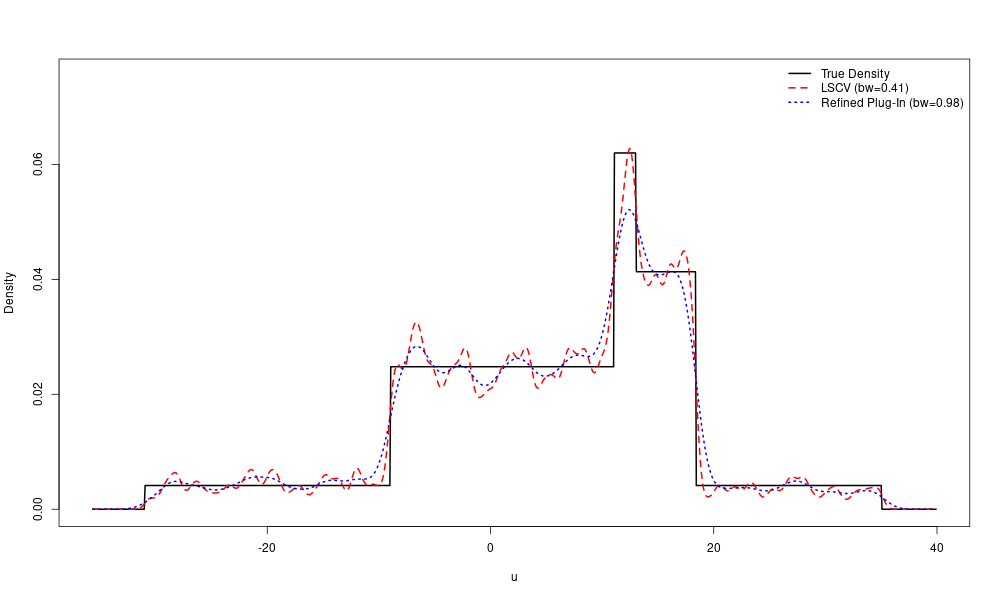
\includegraphics[width=0.8\textwidth]{density_estimation_comparison_p1.png}
  \caption{Density estimation for the mixture distribution, LSCV and Refined Plug\-In methods.}
\end{figure}

\begin{figure}[H]
  \centering
  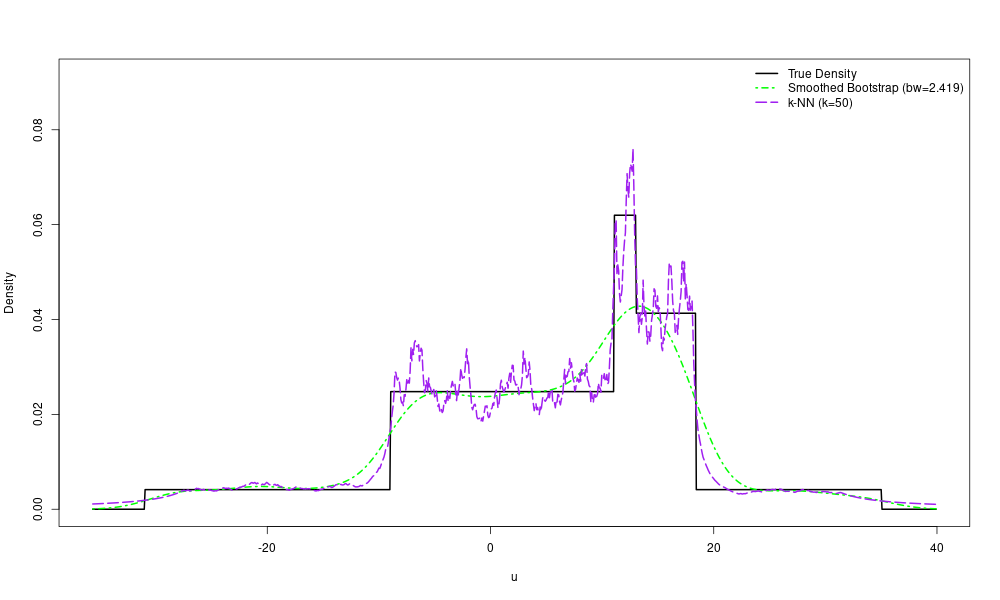
\includegraphics[width=0.8\textwidth]{density_estimation_comparison_p2.png}
  \caption{Density estimation for the mixture distribution, Smoothed Bootstrap and \(k\)-Nearest Neighbor methods.}
\end{figure}

The Integrated Squared Error for each method is as follows:

\begin{table}[H]
\centering
\begin{tabular}{|c|c|}
\hline
\textbf{Method} & \textbf{Integrated Squared Error} \\ \hline
LSCV & 0.000719 \\ \hline
Refined Plug-In & 0.001004 \\ \hline
Smoothed Bootstrap & 0.002104 \\ \hline
\(k\)-Nearest Neighbor & 0.001034 \\ \hline
\end{tabular}
\end{table}

\subsection{Discussion}

The results of the density estimation are as follows:

\begin{itemize}
  \item The LSCV method provides the most accurate density estimate, with the lowest Integrated Squared Error. It captures the general shape of the density and estimates the highest density close to the true density.
  \item The Refined Plug-In method is also accurate, but slightly less so than LSCV. It is smoother than the LSCV method, but it is visibly less accurate in regions of sharp change in the density.
  \item The \(k\)-Nearest Neighbor method is about as accurate as Refined Plug-In, but it is significantly less smooth. Additionally, it estimates the highest density outside the range of the true density.
  \item The Smoothed Bootstrap method captures the general shape of the density, but it is significantly less accurate than the other methods. It is also less smooth and not as accurate in regions of sharp change in the density.
\end{itemize}

\end{document}
